\documentclass[a4paper, 12pt]{article}
\usepackage[left = 2.54cm, right = 2.54cm, top = 2.54cm, bottom = 2.54cm]{geometry}
\setlength{\parindent}{0cm}
\usepackage{graphicx}
\begin{document}
\title{ME20B001}
\author{Aahan Bhargava}
\date{\today}
\maketitle

\tableofcontents

\listoffigures

\section{Aahan Bhargava, ME20B001}
Name: Aahan Bhargava
Roll No.: ME20B001

\section{Equations of choice}
\begin{equation}
\delta Q = dE + \delta W	
\label{eqn:First Law}
\end{equation}

\begin{equation}
S_2-S_1 = \int_{1}^{2}{\delta Q/T} + S_{gen}
\label{eqn:Entropy}
\end{equation}

\subsection{Analysis}
\begin{figure}[h]
	\begin{center}
		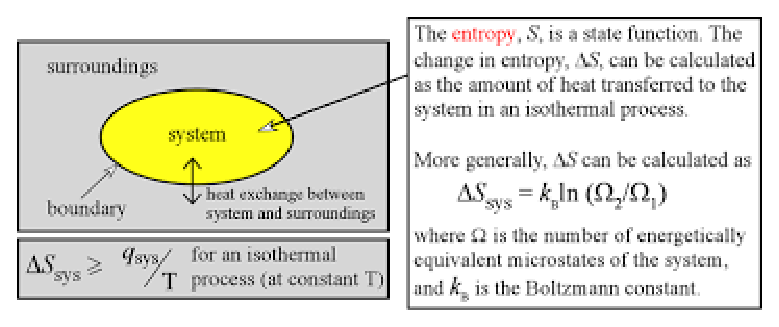
\includegraphics[scale=0.5]{me20b001.eps}
	\end{center}
	\caption{ME20B001}
	\label{entropy}
\end{figure}

Equation~\ref{eqn:First Law} describes the relation of heat(Q) 
work(W) with the energy of a system in differential form.
We have written $ \delta Q $ and $ \delta W $ because heat and work are path functions
and energy(E) is a state function.
Heat and work exchange are important parameters to predict the change in internal energy
of a system.
from~\cite{Myers}.

Equation~\ref{eqn:Entropy} describes the relation between entropy(S), heat(Q)
and Temperature(T). $ S_{gen} $ is the entropy generated because of
irreversibilities in the system, eg: friction.
Entropy is an important parameter to predict the spontaneity of a process.It is a measure
of the randomness of a system.
from ~\cite{Bejan}.

In figure~\ref{entropy} we see the relation between entropy(S), heat(Q) and
Temperatur(T) for any process happening in our world.
 
\bibliography{team-1.bib}
\bibliographystyle{plain}

\end{document}
